\section{Experiments Completed/Scheduled}   \label{sec:experiments}
% Experiments

In order to validate the position control approach proposed in section \ref{sec:technical-approach}, we implement it on two systems. The first is a parallel configuration of three actuators constrained to 2 DOF motion (Figure \ref{fig:modules}a). The second is a parallel combination of four actuators constrained 3 DOF motion (Figure \ref{fig:modules}b).

We choose a set of desired end effector positions, then 

During the experiments, the pressures inside the actuators are varied using pneumatic pressure regulars (Enfield TR-010-g10-s), and the displacement of the end effector is measured using a motion capture system with active trackers (Phase Space Impulse X2E).

%% figure: the 2dor and 3dof rigs, labeled, side to side
\begin{figure}
    \centering
    \begin{tikzpicture}
        \def\colWidth{0.48\linewidth}
        \matrix [row sep=0.5cm, column sep=0cm, style={align=center}] (my matrix) at (0,0)
        {
        \node[style={anchor=center}] {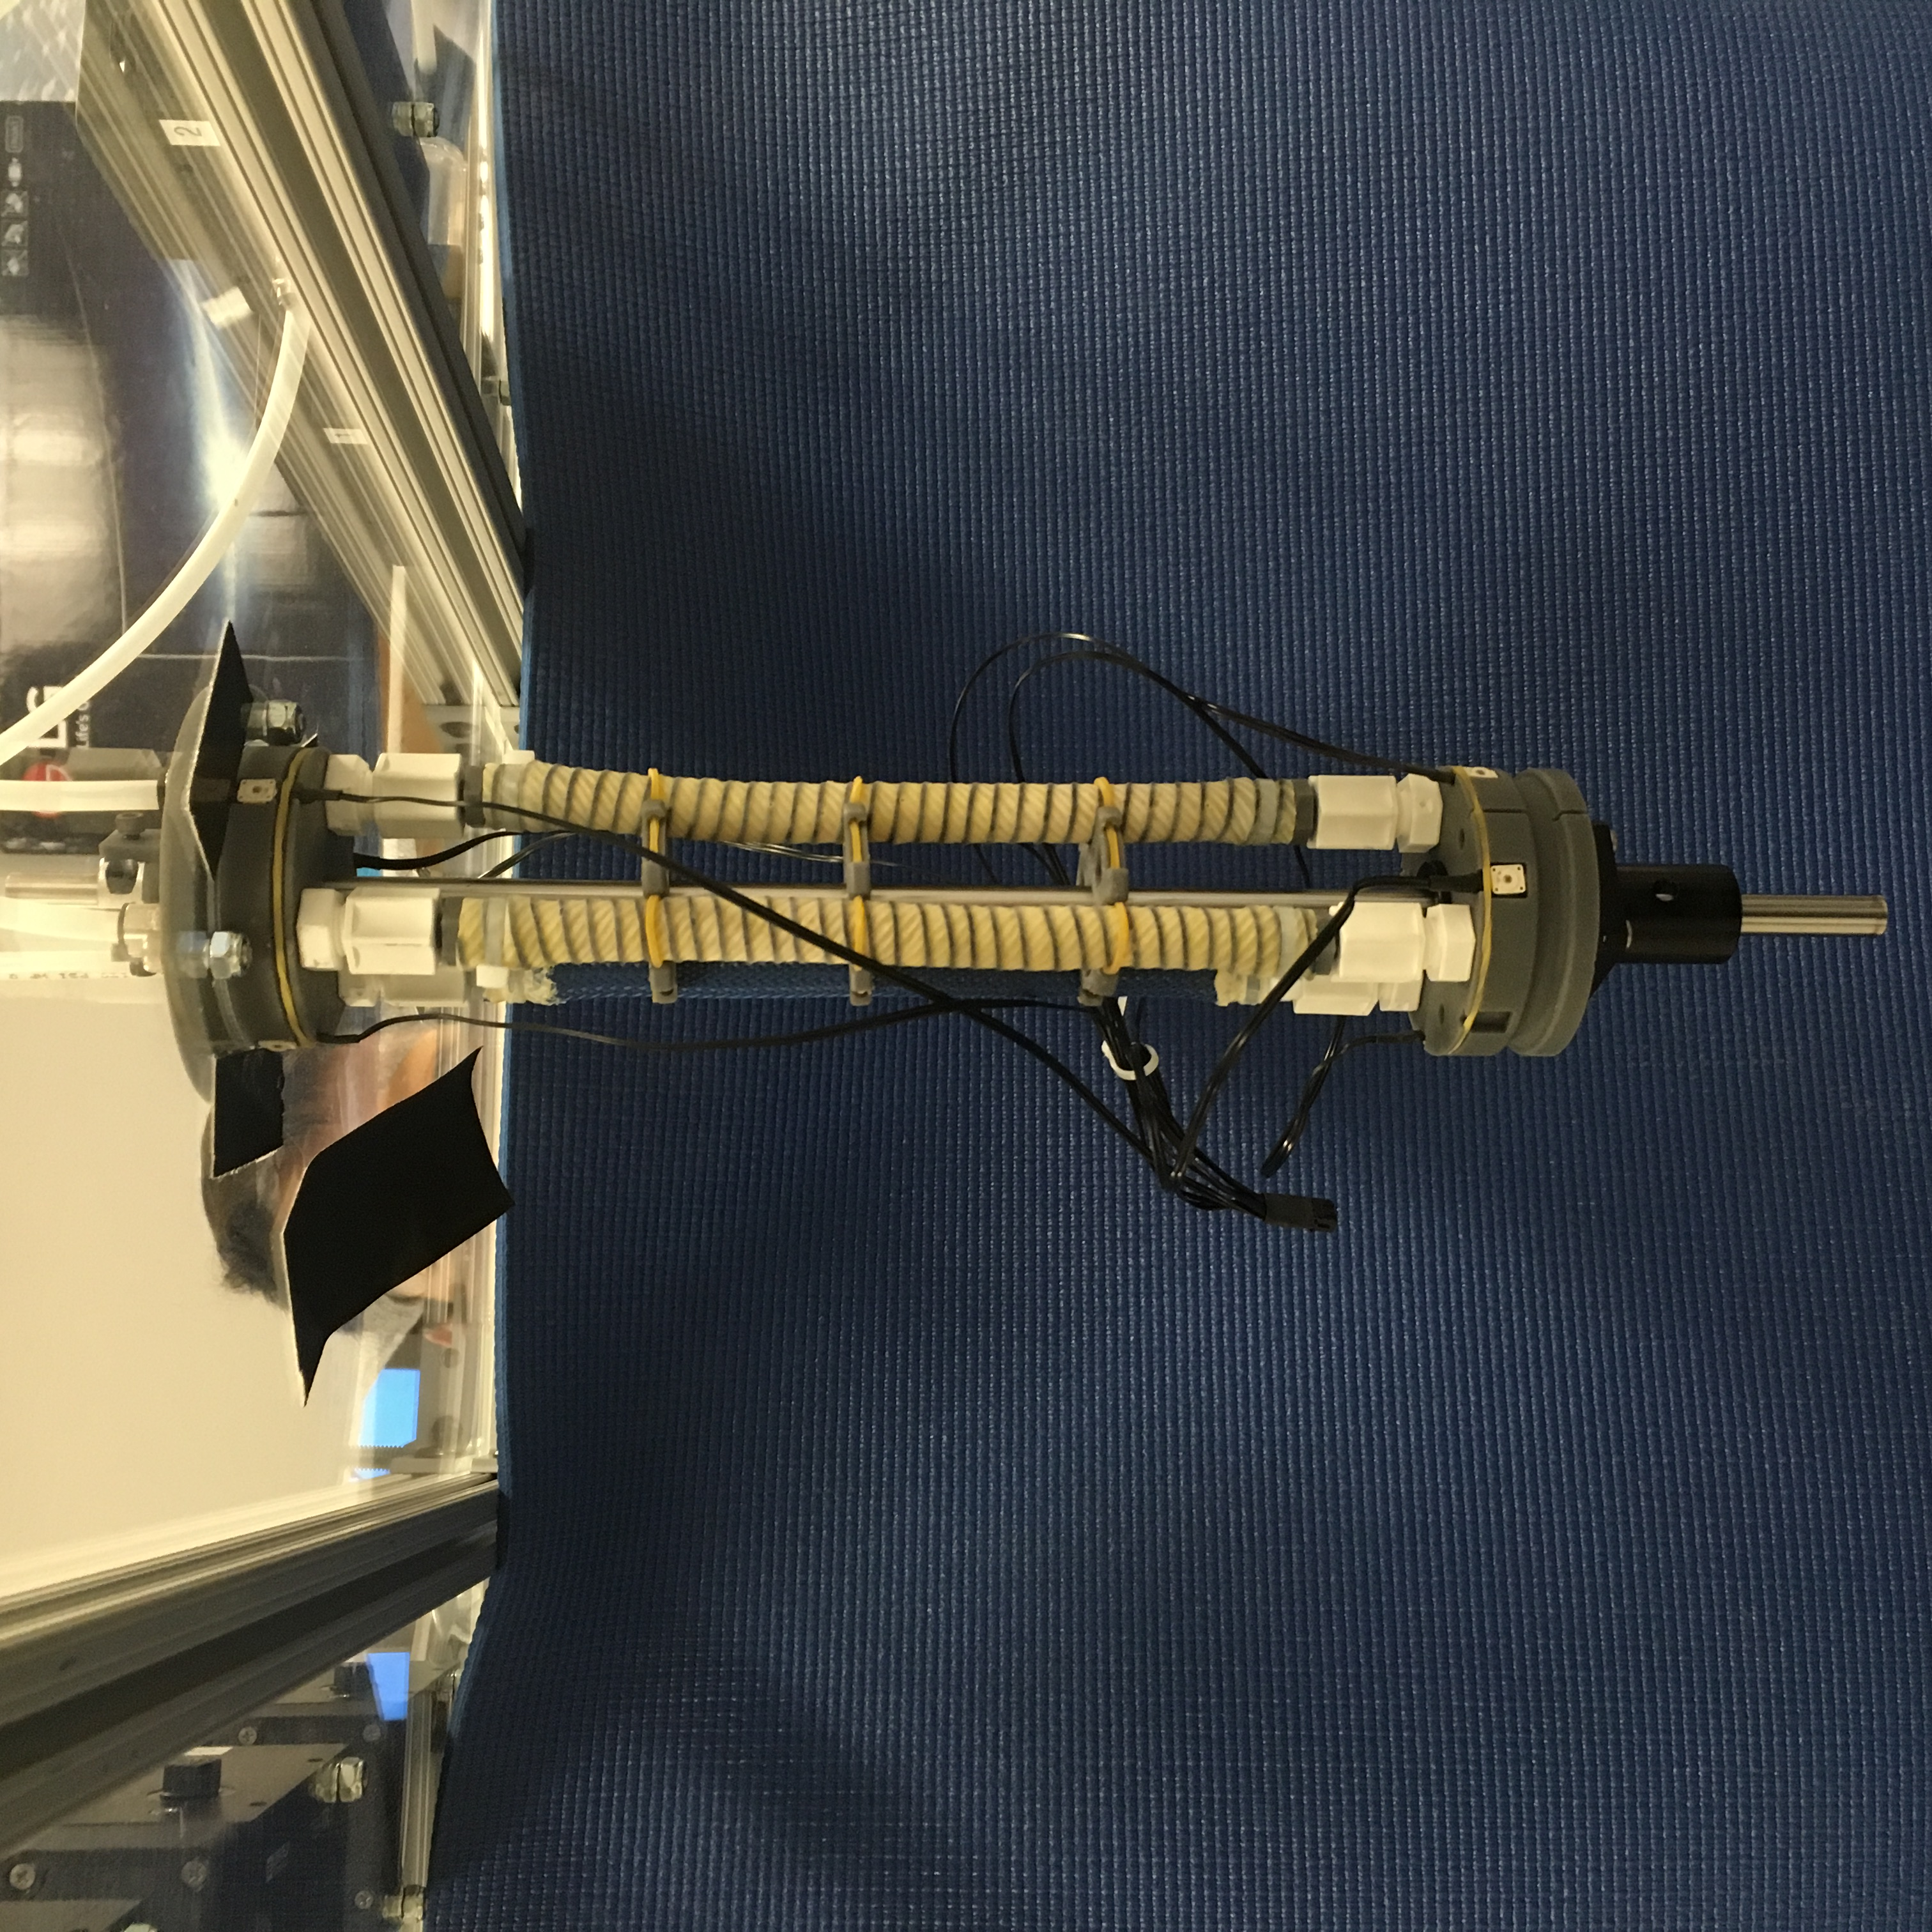
\includegraphics[width=\colWidth, angle=-90]{figures/free3.JPG}};
        &
        \node[style={anchor=center}] {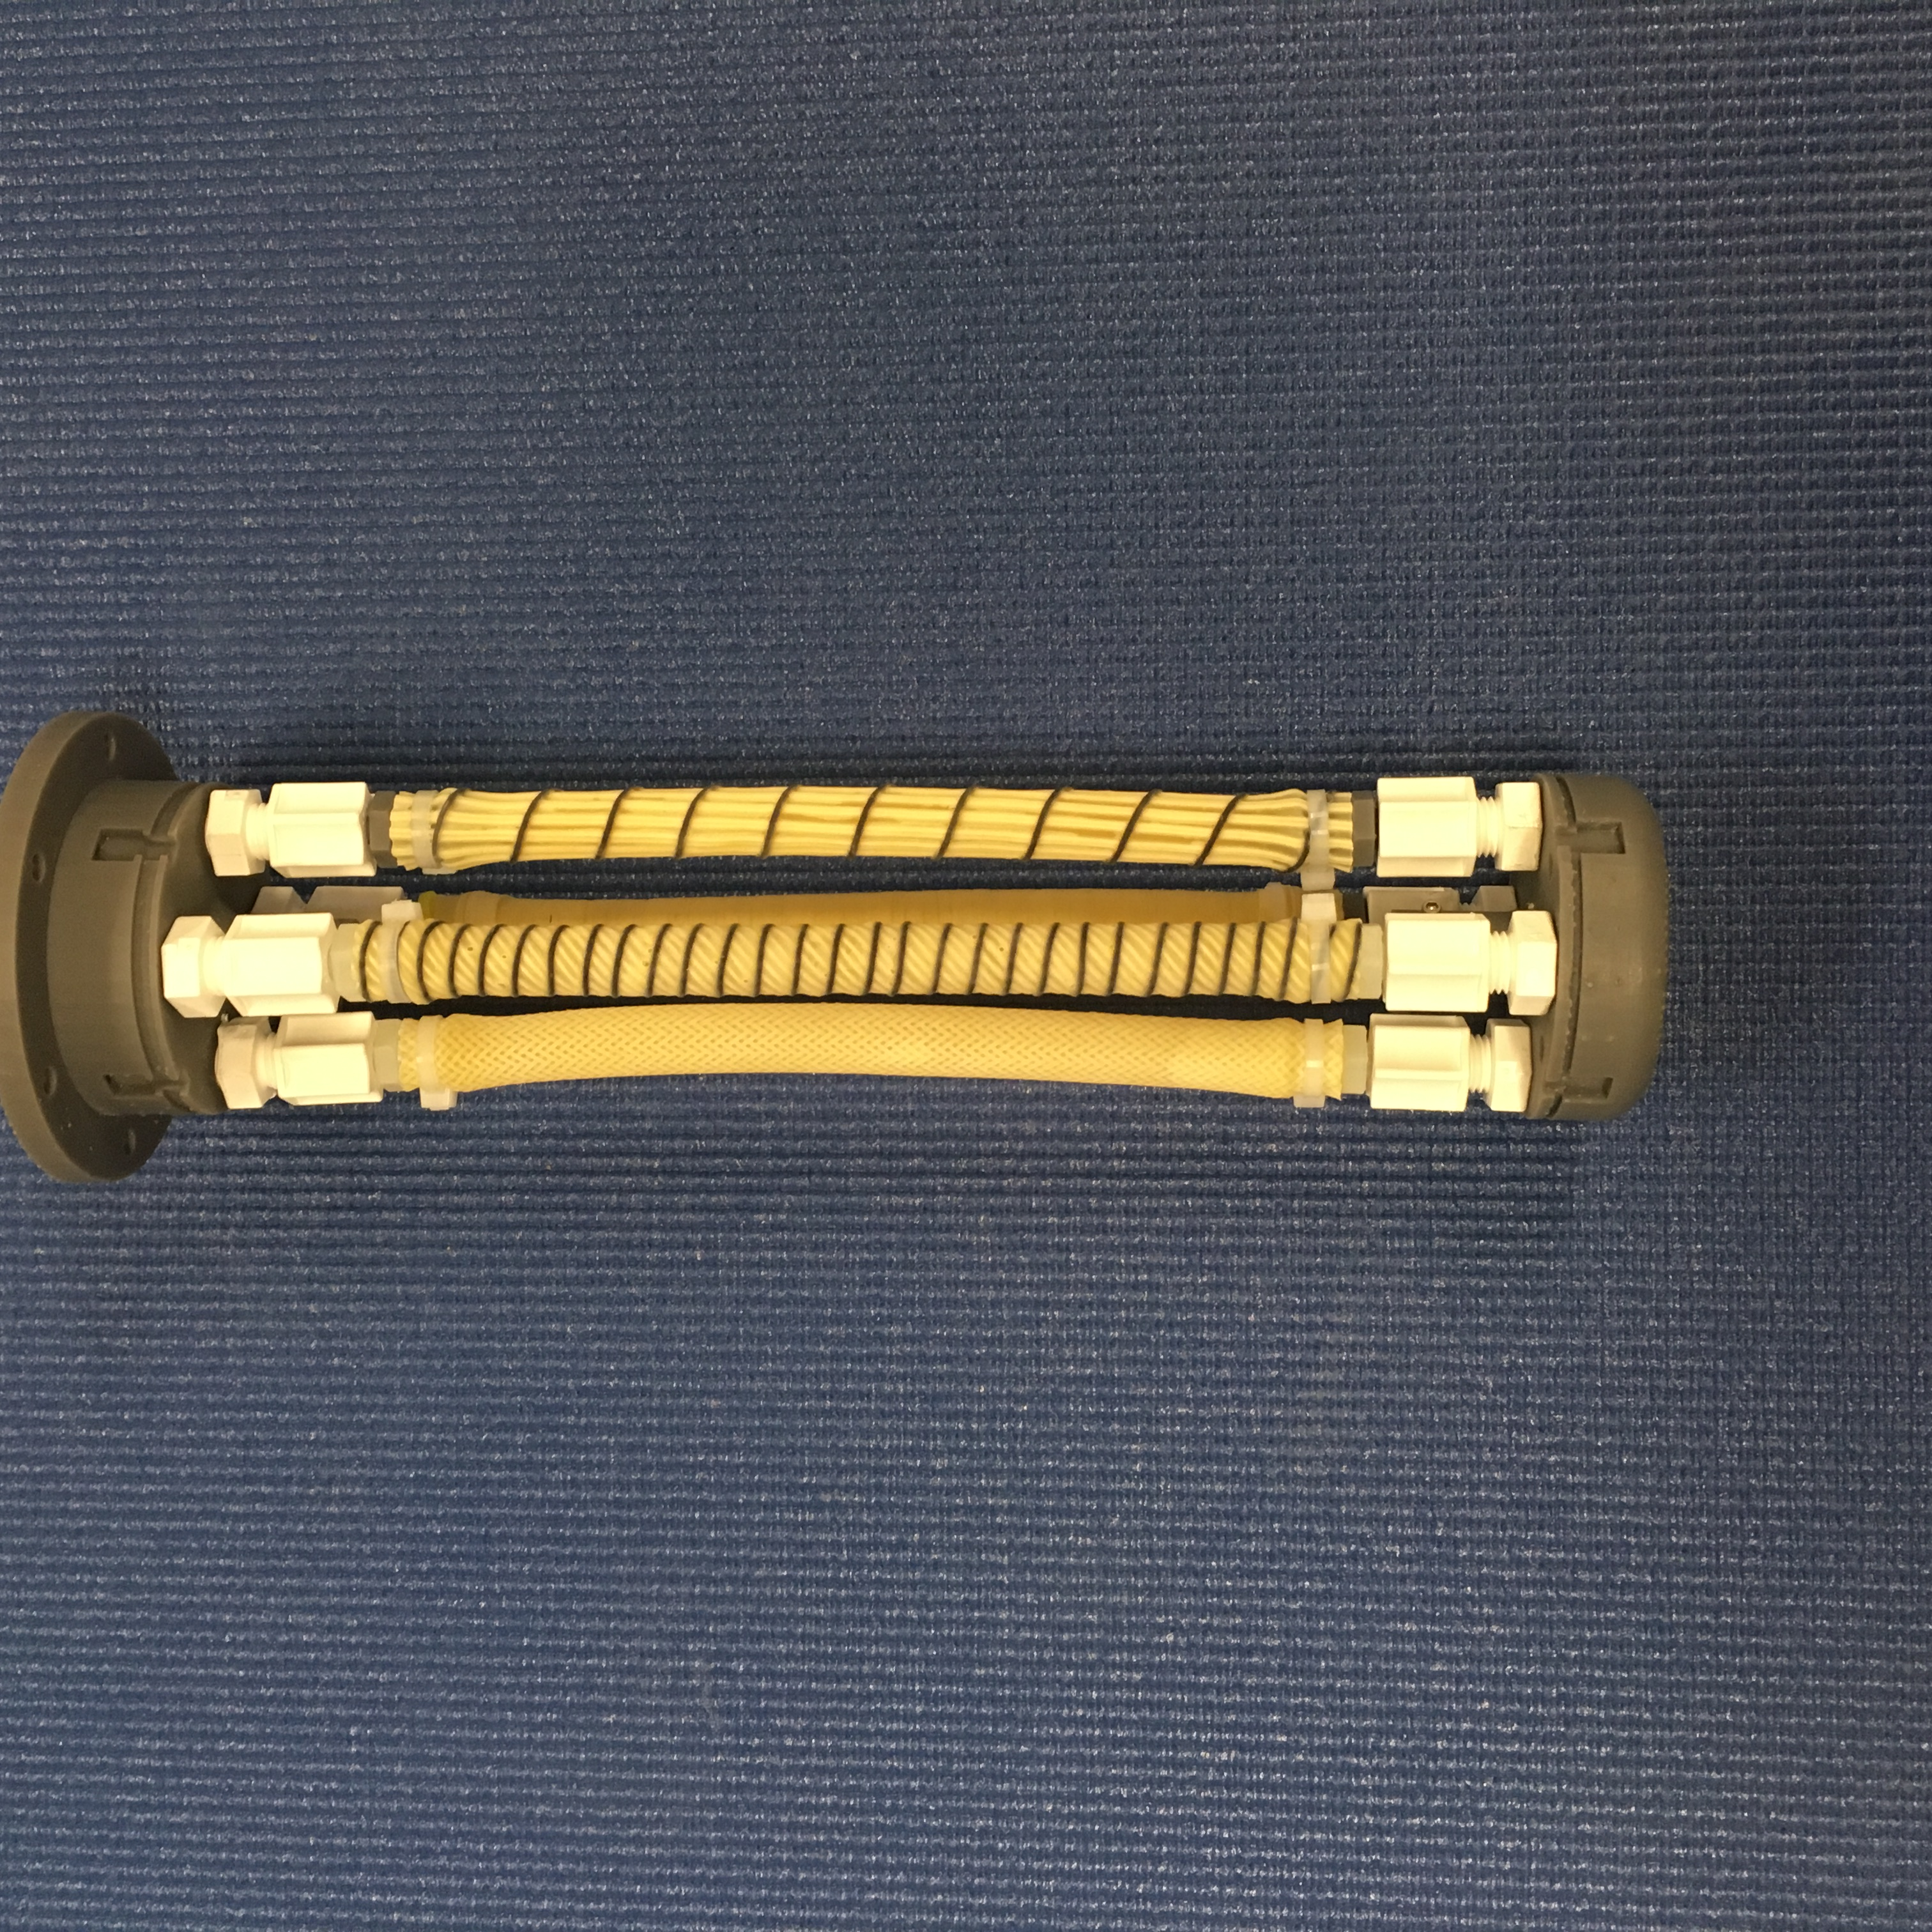
\includegraphics[width=\colWidth, angle=-90]{figures/free4.JPG}};
        \\
        };
    \end{tikzpicture}
    \caption{(a) , (b) . \Dan{these pictures are placeholders. Will be replaced with much nicer versions with labels drawn on to show DOFs.}}
    \label{fig:modules}
\end{figure}

%% Experiments Completed



2DOF translation and rotation experiment. Iterate through a bunch of $\x^\tx{des}$ and compare the measured displacement to that predicted by the model, $\vec{e}_i = \x^\tx{des}_i - \x^\tx{meas}_i$. Then, do the same thing with a torsional load applied. Then do the same thing with unknown loads, but have a feedback loop with a gain on the fload term.

%% figure: 2dof rig in motion capture system


%% Experiments Scheduled

In future experiments we will apply the same approach to the less constrained system shown in figure \ref{fig:modules}b.

%% figure: 3dof compliant spine rig